\documentclass[letter,12pt]{article}
\usepackage[T1]{fontenc}
\usepackage[utf8]{inputenc}
\usepackage{lmodern}
\usepackage{hyperref}
\usepackage[english]{babel}
\usepackage{fourier}
\usepackage[protrusion=true,expansion=true]{microtype}
\usepackage{amsmath,amsfonts,amsthm}
\usepackage[pdftex]{graphicx}
\usepackage{sectsty}								
\usepackage[svgnames]{xcolor}			
%\allsectionsfont{\centering \normalfont\scshape}	
\usepackage{fancyhdr}
\pagestyle{fancyplain}
\fancyhead{}	
\fancyfoot[L]{\small \url{http://toddvance.tech}}		
\fancyfoot[C]{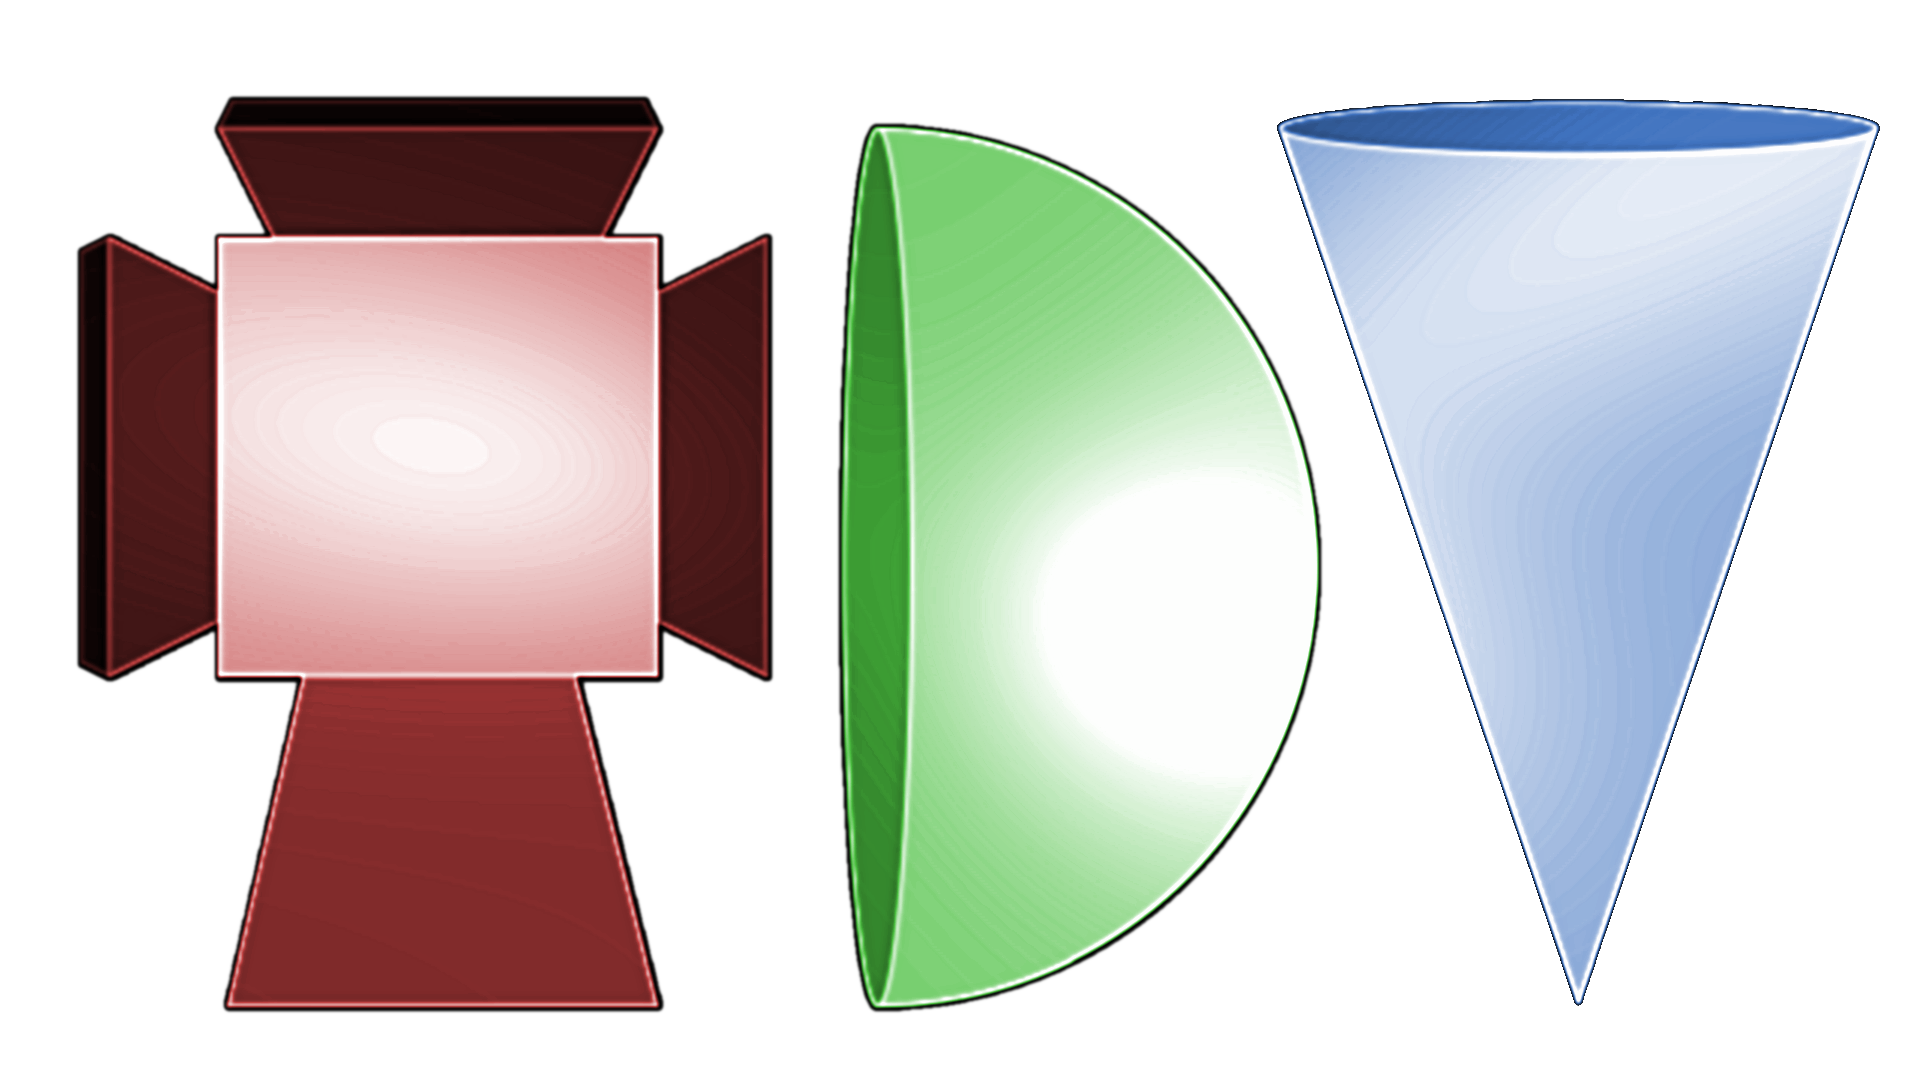
\includegraphics[width=0.5in]{common/monogram-transparent.png}}											
\fancyfoot[R]{\thepage}								
\renewcommand{\headrulewidth}{0pt}			
\renewcommand{\footrulewidth}{0pt}
\setlength{\headheight}{13.6pt}
\newcommand{\horrule}[1]{\rule{\linewidth}{#1}} 	% Horizontal rule

\title{
		%\vspace{-1in}
		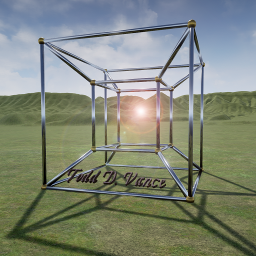
\includegraphics[width=1.5in]{common/tdv-logo-south-branch-valley-small.png}
		\usefont{OT1}{bch}{b}{n} 
		\normalfont 
		\horrule{0.5pt} \\[0.4cm]
		\Huge Pointers\\ %%%%%%%%%%%%%% TITLE %%%%%%%%%%%%%%%
		\color{DarkGreen}
		\large How To\\[0.2cm]%%%%%%%%%%%%%%ARTICLE TYPE %%%%%%%%%%%%%%%
		\color{Blue}
		\small \textsc{Or One Hurdle in Transitioning from Unity to Unreal}\\%%%%%%%%%%%%%% TAG LINE %%%%%%%%%%%%%%%
		\color{Black}
		\horrule{2pt} \\[0.5cm]
}
\author{
		\normalfont \normalsize
       \copyright{2017 Todd D. Vance, Deplorable Mountaineer}%%%%%%%%%%%%%% COPYRIGHT %%%%%%%%%%%%%%%
        \tiny\\
\tiny        Permission is hereby granted, free of charge, to any person obtaining a copy\\[-0.3cm]
\tiny        of this software and associated documentation files (the "Software"), to deal\\[-0.3cm] 
\tiny        in the Software without restriction, including without limitation the rights to\\[-0.3cm]
\tiny         use, copy, modify, merge, publish, distribute, sublicense, and/or sell copies\\[-0.3cm] 
\tiny         of the Software, and to permit persons to whom the Software is furnished to\\[-0.3cm]
\tiny         do so, subject to the following conditions:\\[-0.3cm]
\tiny         \\[-0.3cm]
\tiny	The above copyright notice and this permission notice shall be included in all\\[-0.3cm]
\tiny	copies or substantial portions of the Software.\\[-0.3cm]
\tiny	\\[-0.3cm]
\tiny	THE SOFTWARE IS PROVIDED "AS IS", WITHOUT WARRANTY OF ANY KIND,\\[-0.3cm]
\tiny	EXPRESS OR IMPLIED, INCLUDING BUT NOT LIMITED TO THE WARRANTIES\\[-0.3cm] 
\tiny	OF MERCHANTABILITY, FITNESS FOR A PARTICULAR PURPOSE AND\\[-0.3cm]
\tiny	NONINFRINGEMENT. IN NO EVENT SHALL THE AUTHORS OR COPYRIGHT\\[-0.3cm]
\tiny	HOLDERS BE LIABLE FOR ANY CLAIM, DAMAGES OR OTHER LIABILITY,\\[-0.3cm]
\tiny	WHETHER IN AN ACTION OF CONTRACT, TORT OR OTHERWISE, ARISING\\[-0.3cm]
\tiny	FROM, OUT OF OR IN CONNECTION WITH THE SOFTWARE OR THE USE\\[-0.3cm]
\tiny   OR OTHER DEALINGS IN THE SOFTWARE.
}
\date{\today}

\newtheorem{exercise}{Exercise}

\begin{document}
\maketitle{}
\tableofcontents{}

%%%%%%%%%%%%%% BEGIN DOCUMENT %%%%%%%%%%%%%%%

\section{Introduction}

Pointers are hard.  They are difficult enough that modern languages like Python, Ruby, and Java were designed to not use pointers.  But if you are programming C, C++, and sometimes even C\# (using the “unsafe” code), you will encounter pointers.  Understanding pointers will enrich the understanding of languages that don’t use them, like Python, Ruby, and Java, in the same way that understanding some automobile mechinics enhances the understanding of the car, even when all you do is drive it.  There is a reason that the metaphor “under the hood” is used for some difficult programming concepts, after all.

So, if you are taking the Udemy Unreal course (\url{https://www.udemy.com/unrealcourse/learn/v4/overview}) taught by Ben Tristem and Sam Pattuzzi, you will encounter some lectures on pointers, because writing games for Unreal requires at least some knowledge of pointers.  This HowTo is intended to go beyond the very basics and put a person on a path of “Grokking” (as Robert A. Heinlein would say) pointers “in the fullest”.

The primary prerequisite for this HowTo is a knowledge of some programming language, specifically a knowledge and some experience with arrays.  I shall assume you know how to work with arrays in, for example, C++, or really any language that uses them (which is most languages, Lisp and Assembly being notable exceptions).


\begin{figure}
  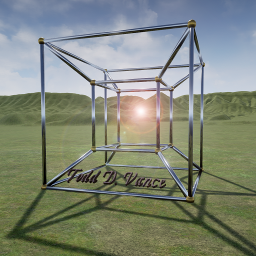
\includegraphics[width=2in]{common/tdv-logo-south-branch-valley-small.png}
  \caption{Hypercube projected into the South Branch Valley}
  \label{fig:logo1}
\end{figure}

\section{Start with Arrays}

Most student programmers are introduced to arrays before being introduced to pointers, because it is easier to understand.  An added advantage is that, pointers can be “modeled” by arrays so this is a big step toward understanding pointers.

In summary, if a variable $a$ is an array then it has some properties (which are specified differently in different languages), the main one being the \emph{length}, sometimes called \emph{dimension}.  So, the following commands define an array of length 10 in various languages:

\begin{itemize}
\item[BASIC:] DIM A(10)
\item[C or C++:] int a[10];
\item[Java:] int[] a = new int[10];
\item[Python:] a = [0]*10;
\end{itemize}

So, arrays have a length.  They also have \emph{elements} indexed by integers.  In BASIC, the elements are 
$A(1)$, $A(2)$, $A(3)$, $A(4)$, $A(5)$, $A(6)$, $A(7)$, $A(8)$, $A(9)$, and $A(10)$.  In the other languages, the elements are $a[0]$, $a[1]$, $a[2]$, $a[3]$, $a[4]$, $a[5]$, $a[6]$, $a[7]$, $a[8]$, and $a[9]$. Since almost all modern languages follow a pattern simimilar to C, C++, Java, and Python, that is what I shall use in this HowTo.  

These are the main properties of arrays.  An array is a single variable that holds an indexed (starting with zero, ending with length - 1 in most langauges) list of values.

Of course, the examples were arrays of integers (except BASIC, where the default is floating point numbers for most dialects).  But arrays in most languages can hold any value, though except for some exceptions like Python, the values must all be the same type.

\section{The Memory Array Using Unity C\#}

Now, let us use arrays to simulate pointers.  I need to pick a language, any language, so how about C\#, which is well-studied in the Udemy course on Unity at \url{https://www.udemy.com/unitycourse/learn/v4/content}.  We shall build a pointer simulator, which hopefully makes real pointers easier to understand.

So, since the Udemy course uses Unity, I shall take the path of least resistance and fire up Unity.  Create a new project called Pointers.  Then, create a new C\# script, also called Pointers (saved in a file called Pointers.cs).  This will be a MonoBehaviour.  So, create a new, empty GameObject in the Hierarchy and attach this new script as a component.

So, now we need an array to represent the memory available to a program. Our simulated pointers will use this array.  The array is declared thus:

\begin{verbatim}
    Object[] memory = new Object[1000];
\end{verbatim}

Put it inside the class definition, but outside of the method definitions like Start and Update.  Thus, the Pointers.cs file will now look something like this:

\begin{verbatim}
using System.Collections;
using System.Collections.Generic;
using UnityEngine;

public class Pointers : MonoBehaviour {

    Object[] memory = new Object[1000];

	// Use this for initialization
	void Start () {
		
	}
	
	// Update is called once per frame
	void Update () {
		
	}
}
\end{verbatim}

In real life, there will be a lot more than 1000 locations for objects, but this is good enough for the simulation.

















\end{document}